\documentclass[11pt, abstracton]{scrartcl}

\usepackage[ngerman]{babel}
\usepackage[T1]{fontenc}
\usepackage[utf8]{inputenc}
\usepackage{lmodern}
\usepackage{graphicx}
\usepackage{amsmath}
\usepackage{biblatex}	
	

\title{Probabilistische Algorithmen}
\subtitle{Seminar Theoretische Informatik}
\author{Thorsten Kober}
\date{16. Juni 2015}


\bibliography{Bibliography}	

\begin{document}

\maketitle

\tableofcontents
\pagebreak


\section{Einführung}


\subsection{Definition}
Unter einem probabilistischen (lat. \emph{probabilis} etwa \emph{glauben, wahrscheinlich}) Algorithmus versteht man ein Verfahren, welches mittels zufälligen Zwischenergebnissen versucht zu einer guten Näherung für ein korrektes Ergebnis zu gelangen.
Er bildet damit das Gegenstück zu einem deterministischen Algorithmus.
\cite{hopcroft_ullman}
\cite{sipser}

\subsection{Hintergrund}	
Es gibt Probleme deren Lösung durch mittels Nichtdeterminismus Vorteile hat, weil:
\begin{itemize}
	\item mit einer deterministischen Umsetzung eine zu Große Laufzeit einhergeht
	\item die Lösung nur \emph{hinreichend gut} und nicht optimal sein muss
	\item eine nichtdeterministische Lösung einfacher zu verstehen oder zu implementieren ist
	\item der Algorithmus nicht deterministische umzusetzen ist
\end{itemize}

Als kleine Motivation jetzt ein Beispiel für einen Algorithmus, dessen probabilistische Umsetzung effizienter ist als eine deterministische. 

\subsection{Beispiel: Quicksort}
\paragraph{Wiederholung:}
Die Vorgehensweise des Quicksort-Algorithmus ist prinzipiell folgende:
\begin{enumerate}
	\item Wähle aus einer Liste unsortierter Elemente eines aus (Pivotelement). Dieses Pivotelement stellt für sich eine einelementige vollständig sortierte Liste da.
	\item Vergleiche alle anderen Elemente der Liste mit dem Pivotelement und füge sie einer neuen Liste $L$ hinzu falls sie kleiner sind als das Pivotelement. Ansonsten füge sie der Liste $R$ hinzu.
	\item Führe Schritt 1 nun mit $L$ und $R$ durch. Enthält eine Liste nur noch ein Element endet der Algorithmus.
	\item Füge die Teillisten nun so zusammen, dass $L$ immer links des jeweiligen Pivotelements steht und $R$ rechts davon. Die resultierende Liste ist nun vollständig aufsteigend sortiert. Absteigend analog mit invertiertem Ordnungskriterium. 
\end{enumerate}
\begin{figure}[h]
	\centering
	\begin{minipage}{.45\textwidth}
		\centering
		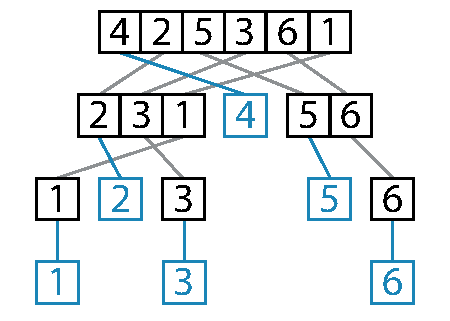
\includegraphics[width=\textwidth]{Graphics/Quicksort_example_avg}
	\end{minipage}
	\begin{minipage}{.45\textwidth}
		\centering
		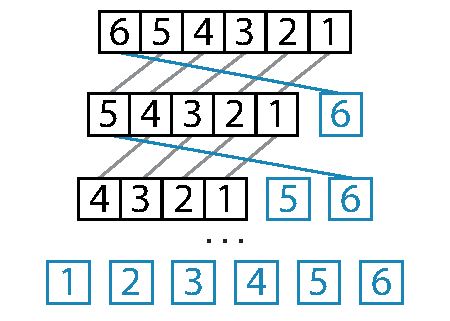
\includegraphics[width=\textwidth]{Graphics/Quicksort_example_wcet}
	\end{minipage}
	\caption{Beispiel für durchschnittliche(links) und schlechteste(rechts) Ausführungszeit eines primitiven Quicksort}
	\label{fig:quicksort_example}
\end{figure}

\paragraph{Beobachtung:}
Die Laufzeit des Quicksort-Algorithmus hängt maßgeblich von der Wahl des Pivotelements ab:
\begin{itemize}
	\item \textbf{Best-Case:} Das Pivotelement wird so gewählt, dass gilt $||L| - |R| | \leq 1$. Daraus ergibt sich mit $log(n)$ Schritten mit je $n$ Vergleichen eine Laufzeit von $\mathcal{O}(nlog(n))$.
	\item \textbf{Worst-Case:} Das Pivotelement wird so gewählt, dass gilt $|L| = 1$ oder $|R| = 1$. Daraus ergibt sich mit $n$ Schritten und je $n$ Vergleichen eine Laufzeit von $\mathcal{O}(n^2)$.
\end{itemize}

\paragraph{Lösung:}
Wird für jede n-elementige Teilliste das Pivotelement zufällig gewählt, beträgt die Wahrscheinlichkeit das schlechteste Element zu wählen $Pr[schlechtestes\ Element\ gewählt] = \frac{1}{n}$.
Selbiges gilt zwar auch für den \emph{Best-Case}, allerdings lässt sich zeigen, dass die Laufzeit der probabilsitischen Variante im Durchschnitt ebenfalls $\mathcal{O}(nlog(n))$ beträgt. \cite{knuth}









\section{Probabilistische Turingmaschinen}
\subsection{Definition}
Wir nutzen das Modell der Mehrband-Turingmaschine um abstrakt die Fähigkeit einer Turing-Maschine zu zeigen, eine zufällige Auswahl zu treffen, entsprechend einem Programm, das einen Zufallszahlengenerator einmal oder mehrfach aufruft.
Auf dem ersten Band steht wie bei einer Mehrband-Turingmaschine üblich die Eingabe.
Das zweite Band, das sogenannte \emph{Zufallsband}, ist vollständig mit den Symbolen $1$ und $0$, die zufällig und unabhängig voneinander mit der Wahrscheinlichkeit $P(x) = \frac{1}{2}, x \in \{0, 1\}$.
Die übrigen Bänder sind initial leer und können nach Bedarf als \emph{Hilfsbänder} genutzt werden.

\begin{figure}[h]
	\centering
	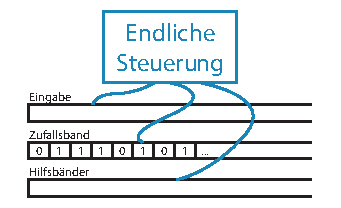
\includegraphics[width=.8\textwidth]{Graphics/Probabilistic_TM}	
	\caption{Darstellung einer zufallsabhängigen Turingmaschine}
	\label{fig:probabilistic_tm}
\end{figure}

Wir nennen dieses Modell einer Turingmaschine \emph{zufallsabhängige Turingmaschine} oder \emph{probabilistische Turingmaschine}.

\paragraph{Bemerkung}
Eine zufallsabhängige Turingmaschine kann als eine Art nichtdeterministische Turingmaschine gesehen werden, bei welcher jeder nichtdeterministische Berechnungsschritt vom Inhalt des Zufallsbandes abhängt.
Einen solchen Berechnungsschritt bezeichnen wir im Folgenden als \emph{Coin-Flip-Schritt}.


\subsection{Initialisierung des Zufallsbandes}
\paragraph{Beobachtung:}
Da die komplette Initialisierung des unendlichen Zufallsbandes mit den Symbolen $1$ und $0$ ist nicht realistisch, da diese nie terminiert.

\paragraph{Lösung:}
Das Zufallsband ist initial ebenfalls leer, enthält also nur \emph{Blanks}. 
Liest der Lese-Schreibkopf auf dem Zufallsband nun ein \emph{Blank}, so wird intern mittels eines Zufallsgenerators eine $1$ oder eine $0$ erzeugt und auf das Zufallsband geschrieben.
Das generierte Symbol wird anschließend nicht wieder verändert.
Auf diese Weise scheint das Zufallsband vollständig initialisiert.


\subsection{Sprache einer zufallsabhängigen Turingmaschine}
Wir sind an Berechnungsmodelle gewöhnt, die immer eine Sprache akzeptieren, zum Beispiel auch $\emptyset$ oder $\Sigma^*$.
Mit dem Begriff der \emph{Akzeptanz} müssen wir bei einer zufallsabhängigen Turingmaschine $M$ etwas vorsichtiger umgehen.
So kann es zum Beispiel vorkommen, dass gar keine Sprache akzeptiert wird.
Es ist sogar möglich, dass $M$ bei gleicher Eingabe und entsprechendem Inhalt auf dem Zufallsband akzeptiert und bei einem anderen Inhalt auf dem Zufallsband nicht akzeptiert.
Dieses Verhalten ist eventuell sogar gewünscht, wenn eine zufallsabhängige Turingmaschine effizienter arbeiten soll als eine deterministische.

Wollen wir eine Aussage über die Verarbeitung einer Eingabe $w$ auf einer zufallsabhängigen Turingmaschine $M$ machen, so müssen wir betrachten wie $M$ sich bei allen möglichen Inhalten des Zufallsbandes verhält.

\paragraph{Definition}
Sei $M$ eine zufallsabhängige Turingmaschine.
Für die Wahrscheinlichkeit einer Berechnung $b$ auf einer Eingabe $w$ gilt
\begin{equation*}
	P(b) = 2^{-k}
\end{equation*}
wobei $k$ die Anzahl der \emph{Coin-Flip-Schritte} in $b$ ist. 
Ferner gilt für die Akzeptanz von $w$
\begin{equation*}
	P(M\ akzeptiert\ w) = \sum_{\substack{b\ ist\ akz.\\ Berechnung}} P(b) 
\end{equation*}

\subsection{Beispiel}
\label{PTM_Example1}
Die folgende Tabelle beschreibt die Übergangsfunktion einer zufallsabhängigen Turingmaschine $M$ mit dem Eingabealphabet $\Sigma = \{a, b\}$, wobei gilt
\begin{description}
	\item [$\boldsymbol{q_i}$] in der Beschriftung der Zeilen bezeichnet einen Zustand mit $q_i \in Q$,
	\item [$\boldsymbol{\rightarrow q_0}$] bezeichnet den Startzustand $q_0 \in Q$,
	\item [$*\boldsymbol{q_i}$] bezeichnet einen Endzustand $q_i \in F$,
	\item [XY] in der Beschriftung der Spalten bezeichnen die gelesenen Symbole auf dem Eingabeband ($X$) und auf dem Zufallsband ($Y$),
	\item [qUVDE] in einer Zelle bedeutet, dass $M$ in den Zustand $q$ wechselt, $U$ auf das Eingabe- und $V$ auf das Zufallsband schreibt und den Eingabekopf in Richtung $D$ sowie den Kopf auf dem Zufallsband in Richtung $E$ bewegt,
	\item [S] als Richtung bedeutet, dass der Kopf auf der aktuellen Position stehen bleibt,
	\item [R] als Richtung bedeutet, dass der Kopf nach rechts bewegt wird.
\end{description}

\bgroup
	\def\arraystretch{1.5}
	\begin{tabular}{r || c | c | c | c | c | c}
		& \textbf{a0} & \textbf{a1} & \textbf{b0} & \textbf{b1} & \textbf{B0} & \textbf{B1} \\
		\hline \hline
		$\boldsymbol{\rightarrow q_0}$ & $q_1a0RS$ & $q_3a1SR$ & $q_2b0RS$ & $q_3b1SR$ & & \\
		\hline
		$\boldsymbol{q_1}$ & $q_1a0RS$ & & & & $q_4B0SS$ & \\
		\hline
		$\boldsymbol{q_2}$ & & & $q_2b0RS$ & & $q_4B0SS$ & \\
		\hline
		$\boldsymbol{q_3}$ & $q_3a0RR$ & & & $q_3b1RR$ & $q_4B0SS$ & $q_4B1SS$ \\
		\hline
		$\boldsymbol{*q_4}$ & & & & & & \\
	\end{tabular}
\egroup

\begin{description}
	\item [a.)] Wie könnte sich $M$ auf der Eingabe $w = ab$ verhalten?
	\item [b.)] Mit welcher Wahrscheinlichkeit akzeptiert $M$ eine homogene Eingabe $a^i,\ i \in \mathbb{N}^+$?
	\item [c.)] Mit welcher Wahrscheinlichkeit akzeptiert $M$ eine heterogene Eingabe? Berechnen Sie $P(M\ akzeptiert\ w),\ w = aabab$! 
\end{description}

\paragraph{Lösungen:}
\begin{description}
	\item [a.)] \ \\
\begin{tikzpicture}[level/.style={sibling distance=4cm/#1}]
	\node (0)[circle,draw]{$q_0$}
  	child {
  		node (12)[circle,draw]{$q_1$} 
  		child {
  			node (21)[circle,draw]{$\times$}
  			edge from parent node[left,draw=none,myblue] {$b0$}
  		}
  		child {
  			node (22)[circle,draw]{$\times$}
  			edge from parent node[right,draw=none,myblue] {$b1$}
  		}
  		edge from parent node[left,draw=none,myblue] {$a0$}
    }
    child {
    	node (11)[circle,draw]{$q_3$}
    	child {
  			node (23)[circle,draw]{$\times$}
  			edge from parent node[left,draw=none,myblue] {$b0$}
  		}
  		child {
  			node (24)[circle,draw]{$q_3$}
  			child {
  				node (31)[circle,draw]{$\checkmark$}
  				edge from parent node[left,draw=none,myblue] {$B0$}
  			}
  			child {
  				node (32)[circle,draw]{$\checkmark$}
  				edge from parent node[right,draw=none,myblue] {$B1$}
  			}
  			edge from parent node[right,draw=none,myblue] {$b1$}
  		}
  		edge from parent node[right,draw=none,myblue] {$a1$}
    };
\end{tikzpicture}
	\item [b.)] $\underbrace{\frac{1}{2}}_{\substack{1.\ Zufallsbit \\ ist\ 0}}\ +\ \underbrace{\frac{1}{2}2^{-i}}_{\substack{1.\ Zufallsbit \\ ist\ 1}} \quad = \quad \frac{1}{2} + 2^{-(i+1)}$
	\item [c.)] $\underbrace{0}_{\substack{1.\ Zufallsbit \\ ist\ 0}}\ +\ \underbrace{\frac{1}{2}2^{-i}}_{\substack{1.\ Zufallsbit \\ ist\ 1}} \quad = \quad 2^{-(i+1)}$ \\ $\Rightarrow\ P(M\ akzeptiert\ w)\ =\ 2^{-6}\ =\ \frac{1}{64}$
\end{description}




\section{Probabilistische Komplexitätsklassen}


\subsection{Wiederholung: Zeitkomplexität}

%\paragraph{Definition}
%Sei $M$ eine Turingmaschine, die immer anhält.
%Die Funktion $f:\mathbb{N}\to\mathbb{N}$ heißt \emph{Zeitkomplexität} von $M$, wobei $f(n)$ die maximale Anzahl an Berechnungsschritten ist.

%\paragraph{Definition}
%Seien $f,g:\mathbb{N}\to\mathbb{N}$.
%Wir schreiben $f(n) = \mathcal{O}(g(n))$ falls gilt:
%\begin{equation*}
%	\forall_{n \geq n_0}:\ f(n)\ \leq \ c \cdot g(n), \quad c \in \mathbb{R}^+,\ n_0 \in \mathbb{N}
%\end{equation*}

%\paragraph{Definition}
%$TIME(t(n))\ =\ \bigl\{L\ \bigl\vert\ \exists TM\ M : M\ entscheidet\ L\ in\ \mathcal{O}(t(n)) \bigl\}$ heißt \emph{Zeitkomplexitätsklasse}.

\paragraph{Definition}
$P = \bigcup\limits_{k=0}^{\infty} TIME(n^k)$ ist die Zeitkomplexitätsklasse der Sprachen, die durch eine deterministische Turingmaschine in polynomieller Zeit entschieden werden können.

%\paragraph{Definition}
%$NTIME(t(n))\ =\ \bigl\{L\ \bigl\vert\ \exists NTM\ M : M\ entscheidet\ L\ in\ \mathcal{O}(t(n)) \bigl\}$ heißt \emph{nichtdeterministische Zeitkomplexitätsklasse}.

\paragraph{Definition}
$NP = \bigcup\limits_{k=0}^{\infty} NTIME(n^k)$ ist die nichtdeterministische Zeitkomplexitätsklasse der Sprachen, die durch eine nichtdeterministische Turingmaschine in polynomieller Zeit entschieden werden können.


\subsection{RP}
\paragraph{Definition}
Sei $M$ eine zufallsabhängige Turingmaschine und $L = L(M)$. $M$ ist vom Typ \emph{Monte Carlo} falls gilt:
\begin{align*}
	Pr[M\ akzeptiert\ w] & = 0,\quad w \notin L \\
	Pr[M\ akzeptiert\ w] & \geq \frac{1}{2},\quad w \in L
\end{align*}
Wir schreiben auch $M$ ist eine \emph{Monte-Carlo-Turinmaschine}.

\paragraph{Definition}
$RP = \bigcup\limits_{k=0}^{\infty} \bigl\{\ L\ \bigl\lvert\ \exists Monte-Carlo-Turingmaschine\ M : M\ entscheidet\ L\ in\ \mathcal{O}(n^k) \bigl\}$ ist die Klasse der Sprachen, die durch eine Monte-Carlo-Turingmaschine in polynomieller Zeit entschieden werden können und wird \emph{Random Polynomial} genannt.

\paragraph{Aufgabe}
Ist die Sprache der zufallsabhängigen Turingmaschine aus dem Beispiel \ref{PTM_Example1} in der Klasse $RP$?

\paragraph{Lösung}
$M$ arbeitet unabhängig vom Inhalt des Zufallsbandes in $\mathcal{O}(n)$ und akzeptiert homogene Eingaben mit einer Wahrscheinlichkeit $\geq \frac{1}{2}$.
Allerdings gibt es heterogene Eingaben die mit einer Wahrscheinlichkeit $< \frac{1}{2}$ akzeptiert werden.
Beispielsweise gilt $Pr[M\ akzeptiert\ w=aab] = 2^{-(3+1)} = \frac{1}{16}$. \\
$\Rightarrow \quad M\ ist\ keine\ Turingmaschine\ vom\ Typ\ Monte\ Carlo$ \\
$\Rightarrow \quad L(M) \notin RP$.

\paragraph{Beobachtung}
Sei $M$ eine Monte-Carlo-Turingmaschine und $L = M(L)$, dann gilt:
\begin{alignat}{2}
	w \notin L \quad & \Rightarrow \quad Pr[M\ akzeptiert\ w] = 0 \\
	w \in L \quad & \Rightarrow \quad Pr[M\ akzeptiert\ w] \geq \frac{1}{2}
\end{alignat}
Offenbar wird $w$ eventuell verworfen obwohl $w \in L$ gilt (\emph{false negative}).
Allerdings wird $w$ nie akzeptiert obwohl $w \notin L$ gilt (\emph{false positive}).

\emph{False negatives} können wir nie vermeiden, aber die Wahrscheinlichkeit ihres Auftretens durch Wiederholung der Prüfung $w \in L$ beliebig minimieren.

\paragraph{Satz}
Sei $L \in RP$, $c > 0$.
\setcounter{equation}{0}
\begin{alignat}
	\exists \exists Monte-Carlo-Turingmaschine\ M:\ 
	& L = L(M), \\
	& Pr[false\ positive] = 0, \\
	& Pr[false\ negative] \leq c, \\
	& M \in \mathcal{O}(n^k) \quad k \in \mathbb{N}^+ 
\end{alignat}

\paragraph{Beweis}
Da $L \in RP$ folgt (1) und (2) aus der Definition von $RP$.
(3) da $M$ eine Turingmaschine vom Typ Monte Carlo ist, gilt per Definition $Pr[M\ akzeptiert\ w] \geq \frac{1}{2}$ falls $w \in L$. \\
$\Rightarrow \quad Pr[false\ negative] \leq \frac{1}{2}$ \\
Die Wahrscheinlichkeit, dass $i$ Prüfungen alle ein \emph{false negative} ergeben ist also $\leq 2^{-i}$. 
Durch $\lceil log_{2}(\frac{1}{c}) \rceil$ Wiederholungen der Prüfung gilt also $Pr[false\ negative] \leq c$. \\
(4) da $L \in RP$ benötigt auch die wiederholte Prüfung einen polynomiellen Zeitaufwand.

\paragraph{Aufgabe}
Sei $L \in RP$. Wie oft muss geprüft werden ob $w \in L$ gilt, damit die Wahrscheinlichkeit eines \emph{false negatives} nicht größer als eins zu eine Milliarde ist?

\paragraph{Lösung}
$\lceil log_{2}(\frac{1}{10^{-9}}) \rceil = 30$

\subsection{BPP}
\paragraph{Definition}
Sei $0 \leq \epsilon < \frac{1}{2}$. Wir sagen \emph{M entscheidet ein wort w mit einem Fehler $\epsilon$} falls gilt:
\begin{align*}
	w \in L \quad & \Rightarrow \quad Pr[M\ akzeptiert\ w] \geq 1 - \epsilon \\
	w \notin L \quad & \Rightarrow \quad Pr[M\ verwirft\ w] \geq 1 - \epsilon
\end{align*}

\paragraph{Definition}
$BPP = \bigcup\limits_{k=0}^{\infty} \bigl\{\ L\ \bigl\lvert\ \exists PTM\ M : M\ entscheidet\ L\ in\ \mathcal{O}(n^k),\ \epsilon =  \frac{1}{3} \bigl\}$ ist die Klasse der Sprachen, die von einer zufallsabhängigen Turingmaschine mit einem Fehler von $\epsilon = \frac{1}{3}$ in polynomieller Zeit entschieden werden können und wird \emph{Bounded-Error Probabilstic Polynomial} genannt.


\subsection{ZPP}
\paragraph{Definition}
Sei $M$ eine zufallsabhängige Turingmaschine und $L = L(M)$. $M$ ist vom Typ \emph{Las Vegas}, wenn sie immer die korrekte Antwort gibt.

\paragraph{Definition}
$ZPP = \bigcup\limits_{k=0}^{\infty} \bigl\{\ L\ \bigl\lvert\ \exists Las-Vegas-Turingmaschine\ M : E(M\ entscheidet\ L) \in \mathcal{O}(n^k) \bigl\}$ ist die Klasse der Sprachen, die durch eine Las-Vegas-Turingmaschine entschieden werden können und für die Zeit bis zum Anhalten einen polynomiellen Erwartungswert hat. 
Sie wird \emph{Zero-Error Probabilitic Polynomial} genannt.


\subsection{Beziehung zwischen ZPP und RP}
\paragraph{Beobachtung}
Offensichtlich gilt $L \in ZPP \Rightarrow \overline{L} \in ZPP$.
Wird nämlich $L$ von einer Las-Vegas-Turingmaschine $M$ mit polynomialem Erwartungswert für den Zeitaufwand akzeptiert, dann wird $L$ von einer modifizierten Las-Vegas-Turingmaschine $M'$ akzeptiert, bei der die Akzeptanz in $M$ durch Anhalten ohne zu akzeptieren, und Anhalten ohne Akzeptanz in $M$ durch Akzeptanz ersetzt wird.

Das $RP$ unter Komplementbildung abgeschlossen ist, ist allerdings nicht offensichtlich.

\paragraph{Definition}
$CoRP = \bigcup \bigl\{\ L\ \bigl\lvert\ \overline{L} \in RP\ \}$

\paragraph{Satz}
$ZPP = RP \cap CoRP$

\paragraph{Beweis}
Zuerst zeigen wir $RP \cap CoRP \subseteq ZPP$.\\
\\
Angenommen $L \in RP \cap CoRP$, dann gibt es für $L$ und $\overline{L}$ Monte-Carlo-Turingmaschinen $M_1$ und $M_2$ in $\mathcal{O}(n^k)$.
Wähle $p(n)$ so, dass $p(n)$ $M_1$ und $M_2$ begrenzt.
Wir entwerfen für $L$ eine Las-Vegas-Turingmaschine $M$ wie folgt:
\begin{enumerate}
	\item $M_1$ akzeptiert $\Rightarrow$ $M$ akzeptiert und hält an.
	\item $M_2$ akzeptiert $\Rightarrow$ $M$ hält an ohne zu akzeptieren.
	\item Wiederhole (1).
\end{enumerate}
Der Erwartungswert für die Ausführungszeit jeder \emph{Runde}(= Schritt (1) und (2)) beträgt $2p(n)$.
Die Wahrscheinlichkeit zu einem Ergebnis zu kommen ist pro Runde $\geq \frac{1}{2}$.
Damit gilt:
\begin{equation*}
	E(M) = 2p(n) + \frac{1}{2}2p(n) + \frac{1}{4}2p(n) + ... = \sum\limits_{k=0}^{\infty}\frac{1}{2^k}2p(n) = 4p(n)
\end{equation*}
$\Rightarrow RP \cap CoRP \subseteq ZPP \hfill \Box$\\
\\
Sehen wir uns nun die Umkehrung an.
Sei $L \in ZPP$.
Wir zeigen $L \in RP$ und $L \in CoRP$.

\paragraph{Teil 1:}
$L \in RP$\\
Wir wissen, es gibt eine Las-Vegas-Turingmaschine $M_A$ mit $L(M_A) = L$ und $E(M_A) = p(n)$.
Wir konstruieren eine Monte-Carlo-Turingmaschine $M_B$ für $L$ wie folgt:
\begin{itemize}
	\item $M_B$ simuliert $w$ auf $M_A$ für $2p(n)$ Schritte, $|w| = n$
	\item $M_A$ akzeptiert $w$ $\Rightarrow$ $M_B$ akzeptiert
	\item sonst verwirft $M_B$
\end{itemize}
Aus dieser Konstruktion folgt:
\begin{align*}
	w \notin L\ &=\ M_A\ akzeptiet\ nicht\ \Rightarrow M_B\ akzeptiert\ nicht \\
	w \in L\ &=\ M_A\ akzeptiet\ ,\ aber\ eventuell\ nicht\ in\ 2p(n)\ Schritten
\end{align*}
Allerdings behaupten wir:
$Pr[M_A\ akzeptiert\ w\ in\ 2p(n)\ Schritten] \geq \frac{1}{2}$ \\
Annahme:
$c = Pr[M_A\ akzeptiert\ w\ in\ 2p(n)\ Schritten] < \frac{1}{2}$ \\
$\Rightarrow\ E(M_A) \geq (1-c)2p(n)$\\
$\xRightarrow{c < \frac{1}{2}}\ 2(1-c) > 1$ und $E(M_A) > p(n) \quad \lightning$\\
$\Rightarrow Pr[M_B\ akzeptiert\ w] \geq \frac{1}{2}$\\
$\Rightarrow M_B\ ist\ vom\ Typ\ Monte\ Carlo$\\
$\Rightarrow L \in RP$

\paragraph{Teil 2:}
$L \in CoRP$\\
Analog mit $\overline{L}$ und $\overline{M_A}$, $\overline{M_B}$.




\section{Beziehungen zwischen RP, BPP und ZPP}
\section{Beziehungenen zu P und NP}
\paragraph{Beobachtung}
Auf den ersten Blick ähneln sich P und ZPP sehr.
Es gilt aber zu beachten, dass für die Sprachen in ZPP lediglich die erwartete Ausführungszeit polynomiell sein muss, während die WCET auch deutlich schlechter sein kann.

\paragraph{Aufgabe}
Welche Beziehung besteht zwischen P und ZPP?

\paragraph{Satz}
$P \subseteq ZPP$

\paragraph{Beweis}
Jede polynomielle deterministische Turingmaschine ist ebenfalls eine polynomielle Las-Vegas-Turinmaschine, die aber ihre Fähigkeit nicht nutzt, eine zufällige Auswahl zu treffen.

\paragraph{Satz}
$RP \subseteq NP$

\paragraph{Beweis}
Wir nehmen an, es gibt eine Monte-Carlo-Turingmaschine $M_1$, $L(M) = L$.
Wir können eine äquivalente, nichtdeterministische Turingmaschine $M_2$ mit gleicher Zeitbegrenzung konstruieren:
\begin{itemize}
	\item $M_2$ \emph{rät} stets das Zufallsbit von $M_1$ und legt es auf ein Hilfsband.
	\item \begin{equation*}
		M_2 =
		\begin{cases}
			akzeptiert &,\ M_1\ akzeptiert\\
			verwirft &,\ sonst
		\end{cases}
	\end{equation*}
\end{itemize}
Folgerung:
\begin{align*}
	w \in &\Rightarrow \text{Es gibt eine erfolgreiche Berechnung, die }M_2\text{ raten kann}\\
	w \notin &\Rightarrow \text{Es gibt keine erfolgreiche Berechnung, die }M_2\text{ raten kann}
\end{align*}

\printbibliography

\end{document}
